\documentclass[a4paper]{article}

%% Language and font encodings
\usepackage[english]{babel}
\usepackage[utf8x]{inputenc}
\usepackage[T1]{fontenc}

%% Sets page size and margins
\usepackage[a4paper,top=3cm,bottom=2cm,left=3cm,right=3cm,marginparwidth=1.75cm]{geometry}

%% Useful packages
%%%%%%%%% begin snippet
%% You need to add the package "tabularx".
%% Place the snippet right after \begin{document}

% need tabularx
\usepackage{tabularx}
\usepackage{amsmath}
\usepackage{graphicx}
\usepackage[colorinlistoftodos]{todonotes}
\usepackage{paralist}
\usepackage{amssymb,amsmath,amsthm,enumitem}
\usepackage[colorlinks=true, allcolors=blue]{hyperref}
\usepackage{subcaption}
\setlength{\abovedisplayskip}{3pt}
\setlength{\belowdisplayskip}{3pt}
\usepackage[hypcap=false]{caption}

\captionsetup{justification=centering}
\captionsetup{format=plain, font=small, labelfont=bf}

\begin{document}
\title{ Computational Intelligence, SS2018 Assignment 2}

\begin{titlepage}
       \begin{center}
             \begin{huge}
				   %% Update assignment number here
                   \textbf{Assignment 2}
             \end{huge}
       \end{center}

       \begin{center}
             \begin{large}
                   Computational Intelligence, SS2018
             \end{large}
       \end{center}

       \begin{center}
 \begin{tabularx}{\textwidth}{|>{\hsize=.33\hsize}X|>{\hsize=.33\hsize}X|>{\hsize=.33\hsize}X|} 

                   \hline
                   \multicolumn{3}{|c|}{\textbf{Team Members}} \\
                   \hline
                   STRUGER & Patrick & 01530664 \\
                   \hline
                   B\"OCK & Manfred & 01530598 \\
                   \hline
                   HAUPT & Anna & 01432018 \\
                   \hline

             \end{tabularx}
       \end{center}

\end{titlepage}

%%%%%%%%% end snippet

\newpage
\tableofcontents
\newpage

\section{Regression with Neural Networks}

\subsection{Simple Regression with Neural Networks}
\begin{enumerate}[label=(\alph*)]
\item \textbf{Learned function}
    In the function ex\_1\_1\_a in file nn\_regression.py:
    \begin{itemize}
        \item Write code to train a neural network on the training set using the regressor method fit, and compute the output predicted on the testing set using the method predict.
        \item Plot the learned functions for $n_h = 2, n_h = 8 ~and ~n_h = 40$ using the test dataset. Use the function plot\_learned\_function in nn\_regression\_plot.py for the plot.
    \end{itemize}
    In your report:    
    \begin{itemize}
        \item Include plots of the learned function and the actual function for all values of $n_h$.
        \item Interpret your results in the context of under/over fitting.
	\end{itemize}

\begin{figure}[htp]
\begin{minipage}{0.4\textwidth}
  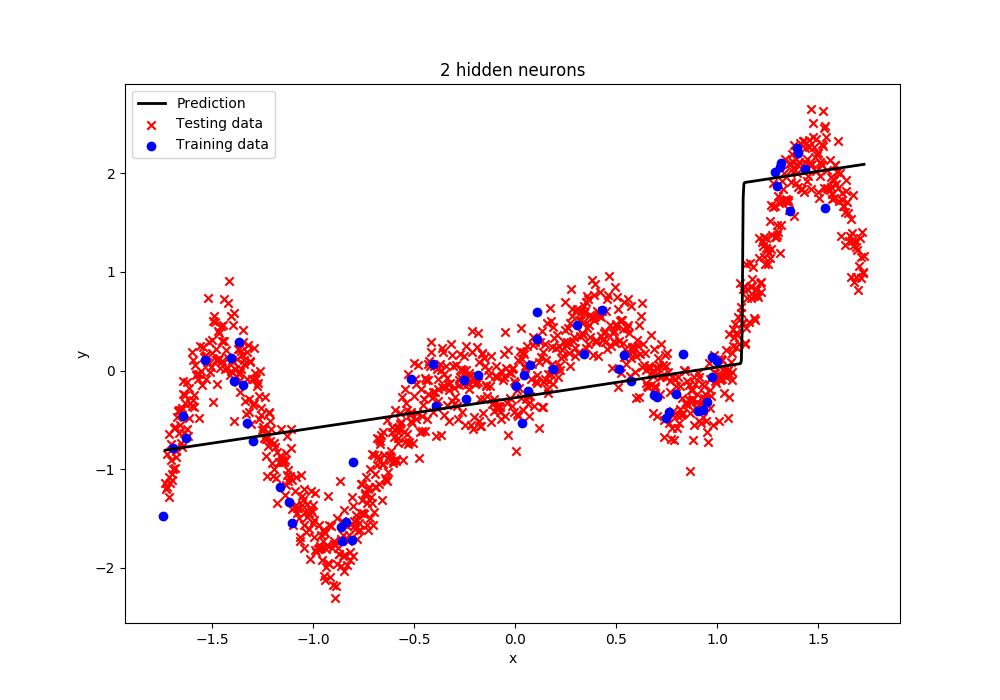
\includegraphics[scale=0.35]{plots/11a_2.png}
  \captionof{figure}{Simple regression with 2 neurons.}
  \label{plot_simple_nh2}
\end{minipage}
\hfill
\begin{minipage}{0.4\textwidth}
  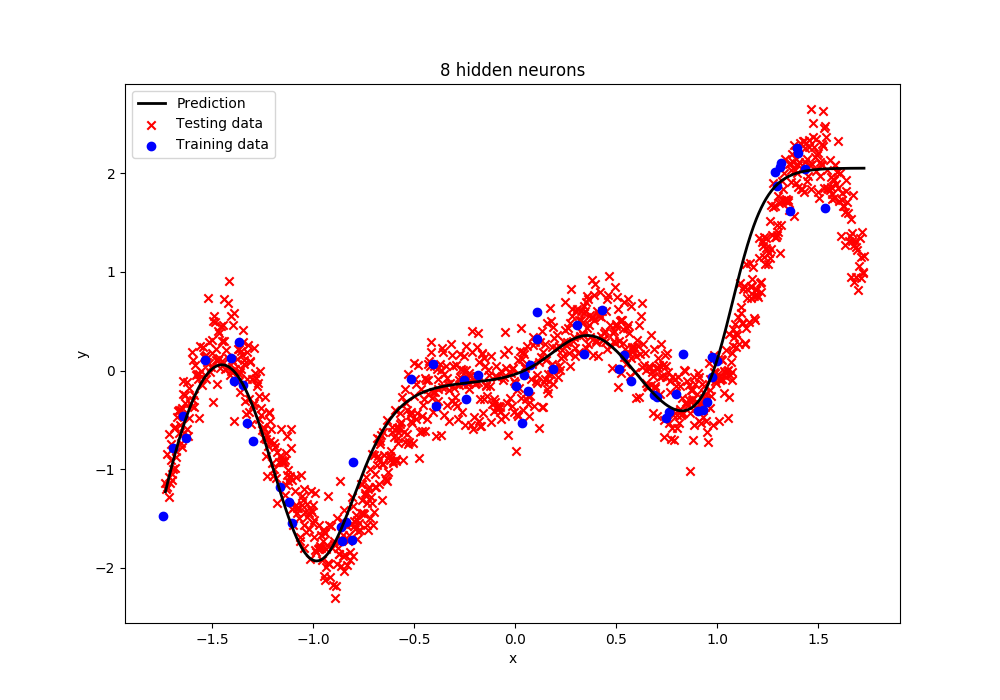
\includegraphics[scale=0.35]{plots/11a_8.png}
  \captionof{figure}{Simple regression with 8 neurons.}
  \label{plot_simple_nh8}
\end{minipage}
\end{figure}

\begin{figure}[htp]
\begin{minipage}{0.4\textwidth}
  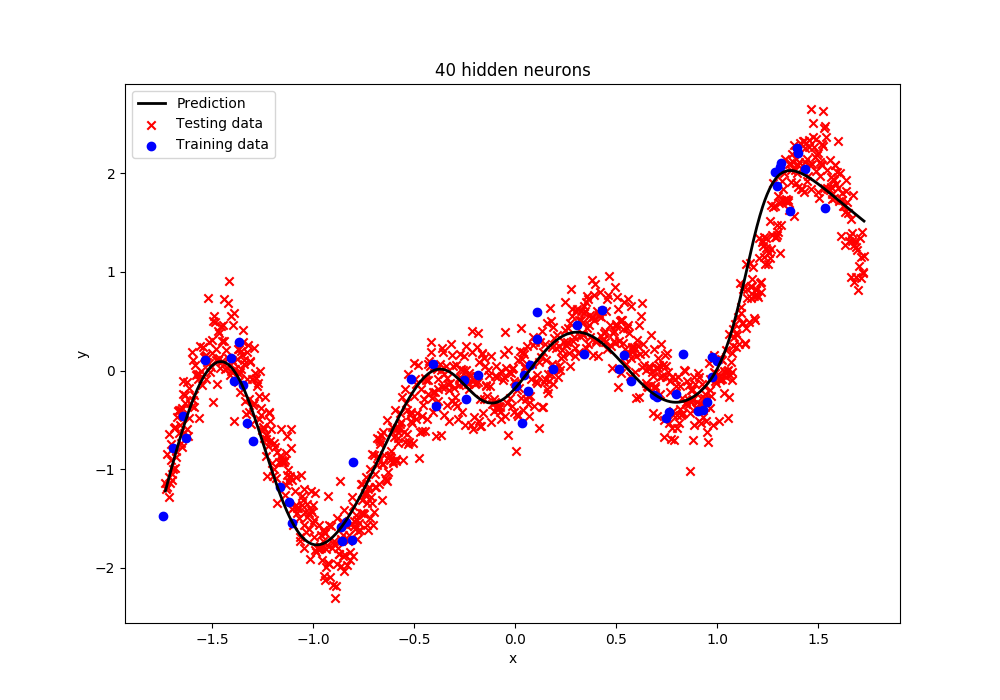
\includegraphics[scale=0.35]{plots/11a_40.png}
  \captionof{figure}{Simple regression with 40 neurons.}
  \label{plot_simple_nh40}
\end{minipage}
\end{figure}

The more hidden neurons are used, the more accuracy in the prediction of the training data occurs. When using fewer neurons it is more likely that the effect of \textit{underfitting} occurs while when using too much neurons the effect of \textit{overfitting} may occur.

\newpage
    
\item \textbf{Variability of the performance of deep neural networks}\\
	In the function calculate\_mse in file nn\_regression.py:
    \begin{itemize}
    	\item Implement the calculation of MSE.
    \end{itemize}
    In the function ex\_1\_1\_b in file nn\_regression.py:
    \begin{itemize}
    	\item Wrap the training together with the MSE evaluations in a for loop, and compute the MSE across 10 different random seeds. Change the random seed by passing a different value to the random\_state argument of the neural network constructor.
    \end{itemize}
	In your report answer the following questions (one sentence is sufficient for each question):

\begin{itemize}
\item \textbf{What is the minimum, maximum, mean and standard deviation of the mean square error obtained on the training set? Is the min MSE obtained for the same seed on the training and on the testing set? Explain why you would need a validation set to choose the best seed?}

\begin{table}[!h]
\centering
\label{ad}
\begin{tabular}{|c|c|c|}
\hline
\textbf{Random Seed} & \textbf{Training Error} & \textbf{Testing Error} \\ \hline
\textbf{1}  &0.05680241   & 0.13079428 \\ \hline
\textbf{2}  &0.0572133   & 0.19897999 \\ \hline
\textbf{3}  &\textcolor{red}{0.0432381}   & 0.20902372 \\ \hline
\textbf{4}  &0.04436419   & \textcolor{red}{0.11277367} \\ \hline
\textbf{5}  &0.05516039   & 0.18864168 \\ \hline
\textbf{6}  &0.05033942   & 0.18287762 \\ \hline
\textbf{7}  &\textcolor{blue}{0.06278832}   & 0.19871679 \\ \hline
\textbf{8}  &0.0627082   & 0.18217017 \\ \hline
\textbf{9}  &0.05904944   & \textcolor{blue}{0.28337206} \\ \hline
\textbf{10} &0.0466659   & 0.19281981 \\ \hline
\end{tabular}
\end{table}

The minimum mean squared error is \textit{0.0432381} using a random seed of 4, while the maximum mean squared error of \textit{0.06278832} occurs when using a random seed of 9. The mean is \textit{0.05383296660111668} and the standard derivation is \textit{0.00688234499225213}.
\newline \newline
As shown in the table above, the minimum MSE for the testing does not indicate the minimum MSE for the training set. It could be very useful to introduce a validation set because it seems to be similar to the testing set. Therefore the validation set indicates the testing set and can be used to find the best matching seed. \\

\item \textbf{Unlike with linear-regression and logistic regression, even if the algorithm converged the variability of the MSE across seeds is expected. Why?}
\newline \newline
That is expected because of the \textit{train-test-split} function, which does not split always the same way (if random state is not set). So the initial weights for calculating the MSE across seeds is not constant. \\

\item \textbf{What is the source of randomness introduced by Stochastic Gradient Descent (SGD)? What source of randomness will persist if SGD is replaced by standard Gradient Descent?}
\newline \newline
In Stochastic Gradient Descent the parameters for every sample observation are estimated (not just the initial one) which gives it a lot of randomness - each sample is evaluated iteratively.
The initial random configuration will persist when replacing SGD by standard Gradient Descent.

\end{itemize}

\newpage

\item \textbf{Varying the number of hidden neurons:}\\
	In the function ex\_1\_1\_c in file nn\_regression.py:
    \begin{itemize}
        \item Write code to train a neural network with $n = [1, 2, 3, 4, 6, 8, 12, 20, 40]$ hidden neurons on one layer. Intialize the regressor with $max_iter=10000, tol=1e-8$.
        \item Compute the MSE over 10 random seeds. Stack the results in an array where the first dimension corresponds to the hidden neuron number and the second dimension indexes the random seed number.
        \item Plot the mean and standard deviation as a function of $n_h$ for both the training and test data using the function plot\_mse\_vs\_neurons in nn\_regression\_plot.py.
		\item Plot the learned functions for one of the models trained with $n_h = 40$ (make sure you use $max_iter=10000, tol=1e-8$). Use the function plot\_learned\_function in nn\_regression\_plot.py for the plot.
    \end{itemize}
    In your report:
    \begin{itemize}
\item \textbf{What is the best value of $n_h$ independently of the choice of the random seed?}
\newline
The best amount of neural networks we obtained is 6. \\

\item \textbf{Include plots of how the MSE varies with the number of hidden neurons.}
\begin{figure}[htp]
\centering
\begin{minipage}{0.4\textwidth}
  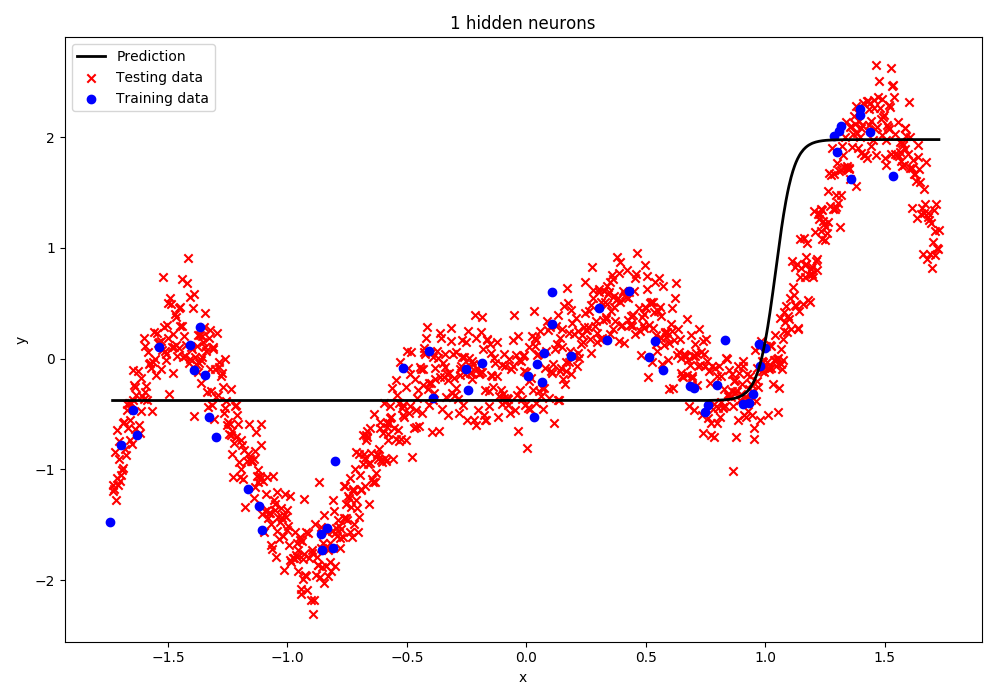
\includegraphics[scale=0.25]{plots/11c_1.png}
  \captionof{figure}{Regression with 1 neuron \\ $\rightarrow$ \textit{underfitting}.}
  \label{plot_simple_nh2}
\end{minipage}
\hfill
\begin{minipage}{0.4\textwidth}
  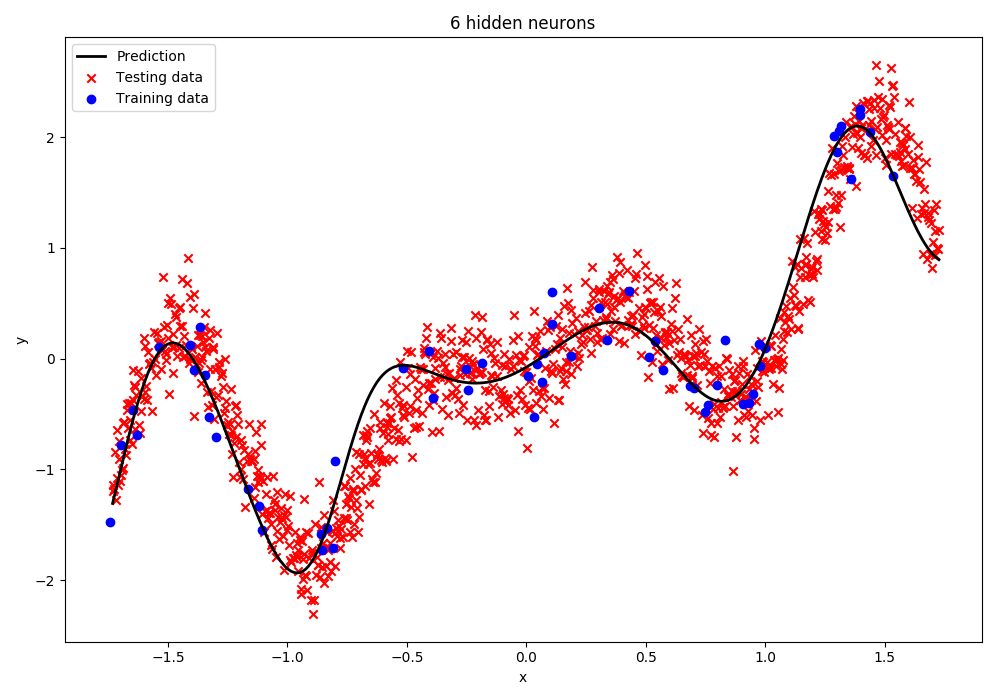
\includegraphics[scale=0.25]{plots/11c_6.png}
  \captionof{figure}{Regression with 6 neuron \\ $\rightarrow$ \textit{mostly accurate}.}
  \label{plot_simple_nh8}
\end{minipage}
\end{figure}

\begin{figure}[htp]
\centering
\begin{minipage}{0.4\textwidth}
  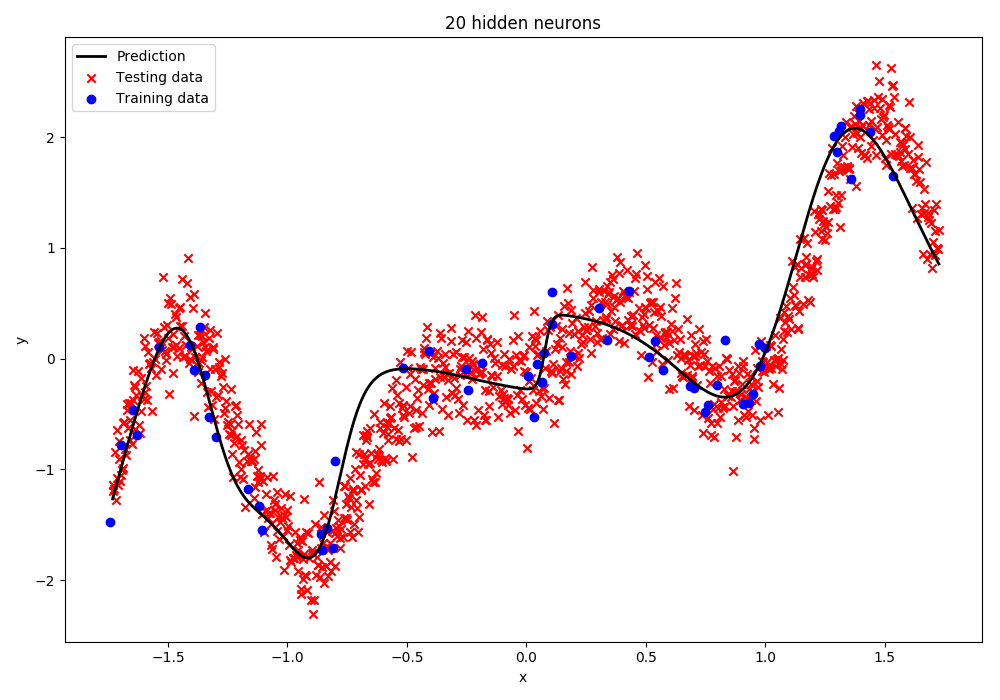
\includegraphics[scale=0.25]{plots/11c_20.png}
  \captionof{figure}{Regression with 20 neuron \\ $\rightarrow$ \textit{overfitting}}
  \label{plot_simple_nh2}
\end{minipage}
\hfill
\begin{minipage}{0.4\textwidth}
  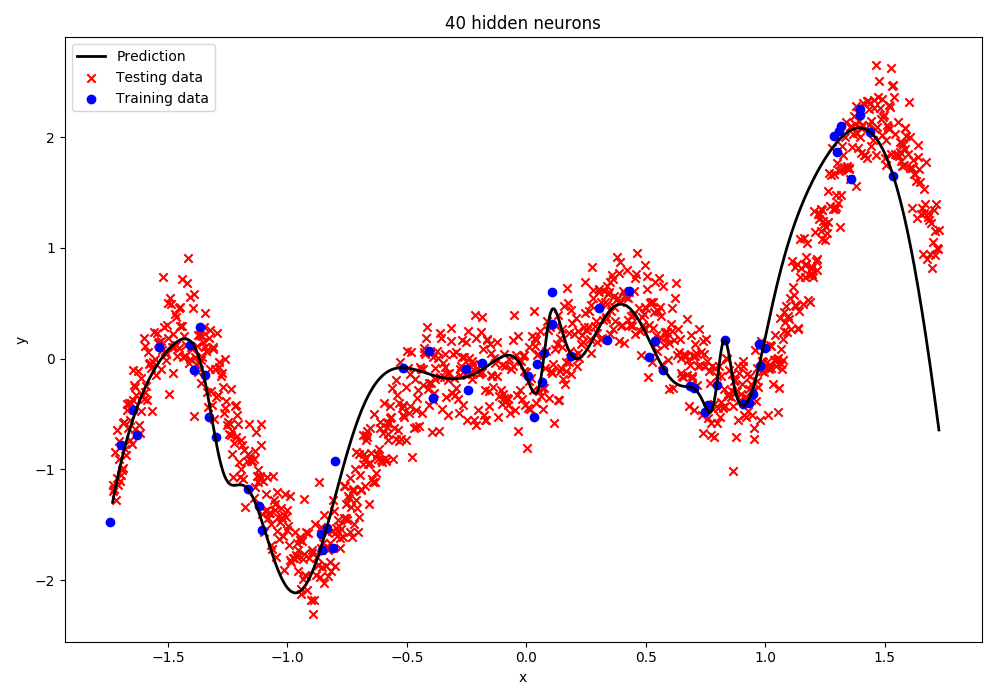
\includegraphics[scale=0.25]{plots/11c_40.png}
  \captionof{figure}{Regression with 40 neuron \\ $\rightarrow$ \textit{overfitting}}
  \label{plot_simple_nh8}
\end{minipage}
\end{figure}

\newpage

\item \textbf{Interpret and discuss your results in the context of over/under fitting}
\newline \newline
When using neurons under 6, we got the problem of underfitting, while when using more than 40 neurons the effect of overfitting may occur.
\end{itemize}
    
\begin{figure}[htp]
  \centering
  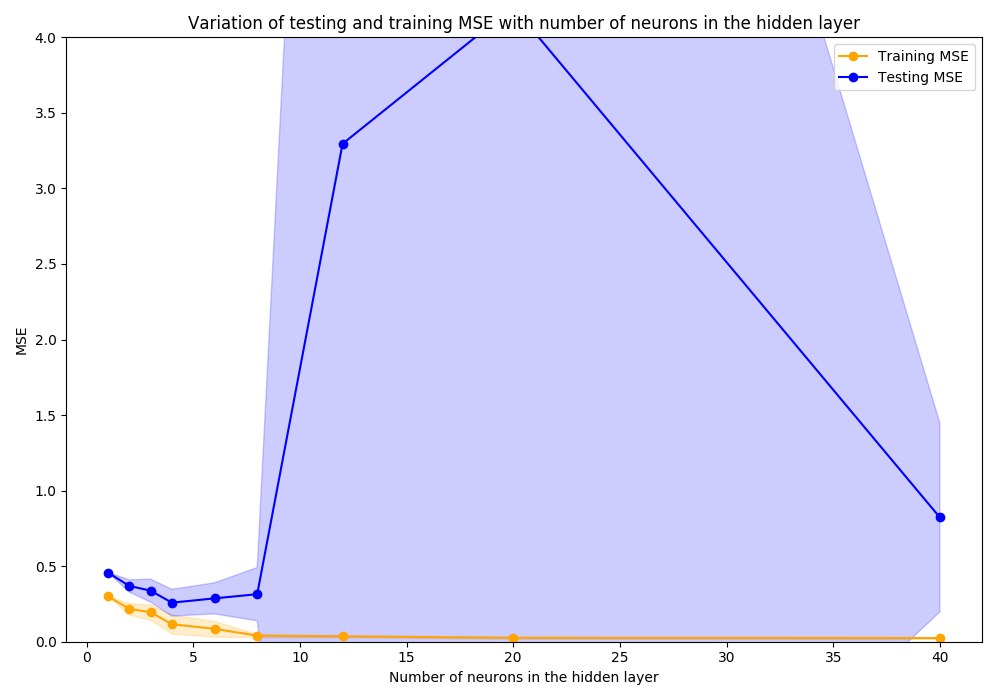
\includegraphics[scale=0.35]{plots/11c_mseVSneurons.png}
  \captionof{figure}{The mean and standard deviation as a function of $n\_{h}$ for both the training and test data.}
  \label{plot_simple_nh}
\end{figure}
\hfill

\item \textbf{Variations of MSE during training:}\\
In the function ex\_1\_1\_d in file nn\_regression.py:
\begin{itemize}
\item Write code to train a neural network with $n_h ∈ 2, 8, 40$ hidden neurons on one layer and calculate the MSE for the testing and training set at each training iteration for a single seed, say $0$. To be able to calculate the MSEs at each iteration, set warm\_start to True and max\_iter to $1$ when initializing the network. The usage of warm\_start always keeps the previously learnt parameters instead of reinitializing them randomly when fit is called. Then, loop over  iterations and successively call the fit function and calculate the MSE on both datasets. Use the training solver ‘lbfgs’, for 10000 iterations. Stack the results in an array with where the first dimension correspond to the number of hidden neurons and the second correspond to the number of iterations Use the function plot\_mse\_vs\_iterations in nn\_regression\_plot.py to plot the variation of MSE with iterations.
        \item Replace the solver by ‘sgd’ or ‘adam’ and compute the MSE across iterations for the same values of $n_h$.
	\end{itemize}
    In your report, answer the following questions:
    \begin{itemize}

\item \textbf{Is the risk of overfitting increasing or decreasing with the number of hidden neurons?}
\newline \newline
In our case lbfgs seems to be perform best.
\newline Overfitting increases with the number of hidden neurons.

\newpage

\item \textbf{‘adam’ is a variant of ‘sgd’ and both are first order methods (the parameter updates are based on the gradient only), whereas ‘lbfgs’ is a second order method (the updates are also based on the Hessian). Which methods seem to perform best in this problem ? What feature of stochastic gradient descent helps to overcome overfitting ? The neural network is rather small as compared to what is used is real-life problems, according to your analysis which solver will be more appropriate when the number of neurons increases?}
\newline \newline
To overcome overfitting are the regularization parameter alpha, early stopping or mini-batch learning is used.
If the number of neurons increases first order methods are more appropriate (e.g adam solver). \\

\item \textbf{Include the plot of the variations of the MSE with three different number of hidden neurons for each solver.}

\begin{figure}[htp]
\begin{minipage}{0.4\textwidth}
  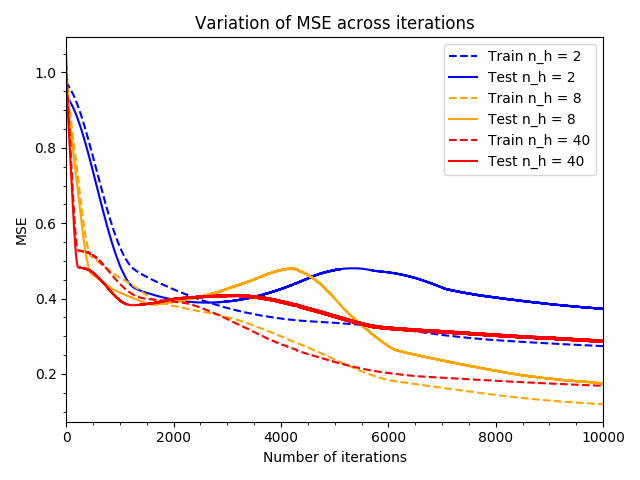
\includegraphics[scale=0.35]{plots/11d_adam.png}
  \captionof{figure}{Variation with  Adam Solver.}
  \label{plot_simple_nh2}
\end{minipage}
\hfill
\begin{minipage}{0.4\textwidth}
  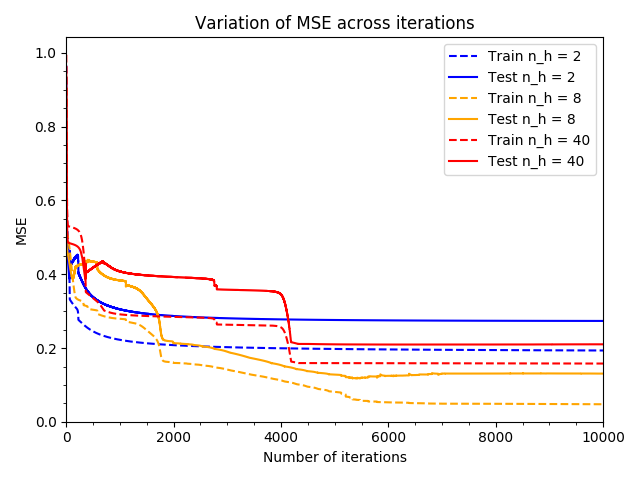
\includegraphics[scale=0.35]{plots/11d_lbfgs.png}
  \captionof{figure}{Variation with Lbfgs Solver.}
  \label{plot_simple_nh8}
\end{minipage}
\end{figure}

\begin{figure}[htp]
\begin{minipage}{0.4\textwidth}
  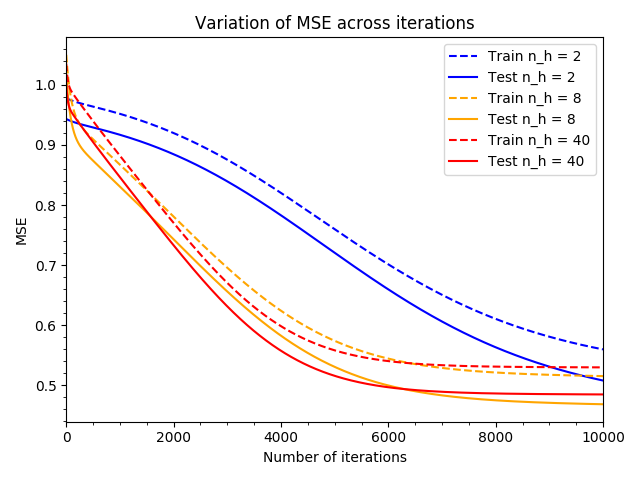
\includegraphics[scale=0.35]{plots/11d_sgd.png}
  \captionof{figure}{Variation with Sgd Solver.}
  \label{plot_simple_nh40}
\end{minipage}
\end{figure}

\end{itemize}         
\end{enumerate}

\newpage

\subsection{Regularized Neural Networks}
Now we want to investigate different regularization methods for neural networks, i.e. weight decay and early stopping. Use the same dataset as before.

\begin{enumerate}[label=(\alph*)]
	\item \textbf{Weight Decay:}\\
    Here, we train the network with different values of the regularization parameter $\alpha$. The loss function in this case looks like this:
    \[
    	msereg = mse + \frac{\alpha}{2n}\sum_i w_i^2
    \]
    In the function ex\_1\_2\_a in file nn\_regression.py:
    \begin{itemize}
        \item Write code to train a neural network with $n = 40$ hidden neurons with values of alpha $\alpha = [10−8, 10−7, 10−6, 10−5, 10−4, 10−3, 10−2, 10−1, 1, 10, 100]$. Stack your results in an array where the first axis correspond to the regularization parameter and the second to the number of random seeds. Use the training solver ‘lbfgs’, for 200 iterations and 10 different random seeds.
        \item Plot the variation of MSE of the training and test set with the value of $\alpha$. Use the function plot\_mse\_vs\_alpha in nn\_regression\_plot.py to plot the MSE variation with $\alpha$.
    \end{itemize}
In your report:
\begin{itemize}
\item \textbf{Include plots of the variation of MSE of the training and test set with the value of $\alpha$.}

\begin{figure}[htp]
  \centering
  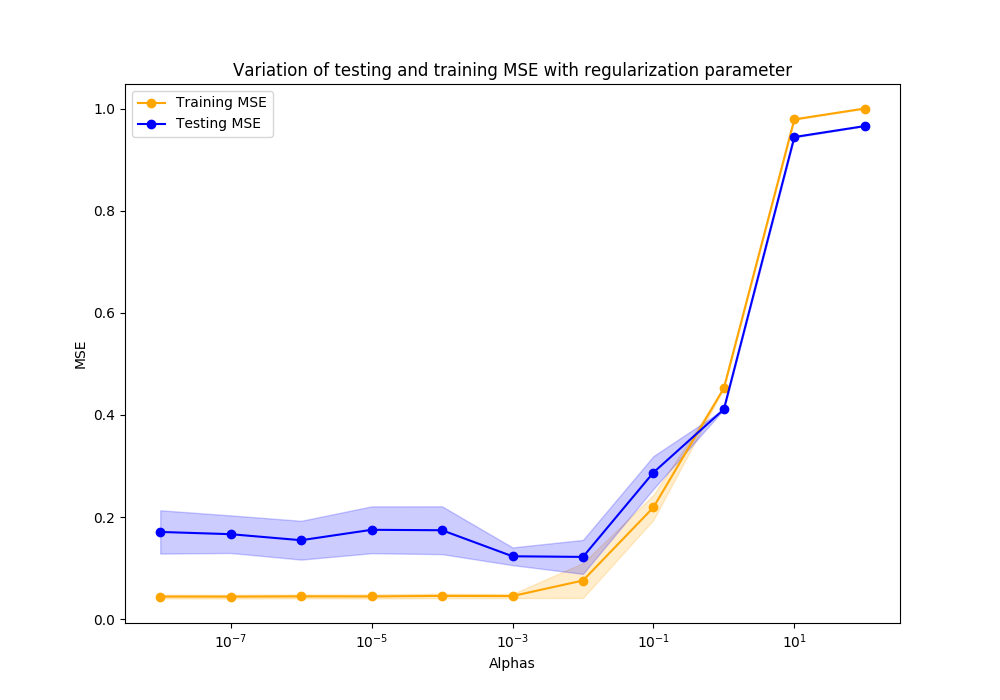
\includegraphics[scale=0.50]{plots/12a.png}        \caption{Variation of MSE of the training and test set with the value of $\alpha$.}
  \label{fig:12a}
\end{figure}

\item \textbf{What is the best value of $\alpha$?} \\
The best value for $\alpha$ seems to be $10^{-2}$. \\

\item \textbf{Is regularization used to overcome overfitting or underfitting? Why?} \\
Regularization is used to keep the value of the regularization parameters as small as possible. Therefore it is used to overcome overfitting because it prefers simple models.
\end{itemize}

\newpage

    \item \textbf{Early Stopping:}\\
    This question demonstrates how early stopping is very efficient at reducing overfitting. To put ourself in extreme overfitting condition, we add some noise to the training data. This is already done in nn\_regression\_main.py.\\
	In the function ex\_1\_2\_b in file nn\_regression.py:
    \begin{itemize}
        \item Early stopping requires the definition of a validation set. Split your training set so that half of your old training set become your new training set and the rest is your validation set. Watch out, it is crucial to permute the order of the training set before splitting because the data in given in increasing order of $x$.
        \item Write code to train a neural network with $n = 40$ and $\alpha = 10−3$ on each selection of the training set. Train for 2000 iterations using the ‘lbfgs’ solver for 10 different random seeds and monitor the error on each set every 20  iterations. For each individual seed, generate the list of (1) the test errors after the last iteration, (2) the test errors when the error is minimal on the validation set, (3) the ideal test error when it was minimizing the error on the test set.
        \item Use the function plot\_bars\_early\_stopping\_mse\_comparison in nn\_regression\_plot.py to plot bar plats comparing MSE for early stopping with last iteration and the ideal case.
    \end{itemize}
In your report: 
\begin{itemize}
\item \textbf{Include the bar plots to compare the errors on the test sets at the last training iterations, at early stopping and when it is minimal.}

\begin{figure}[htp]
  \centering
  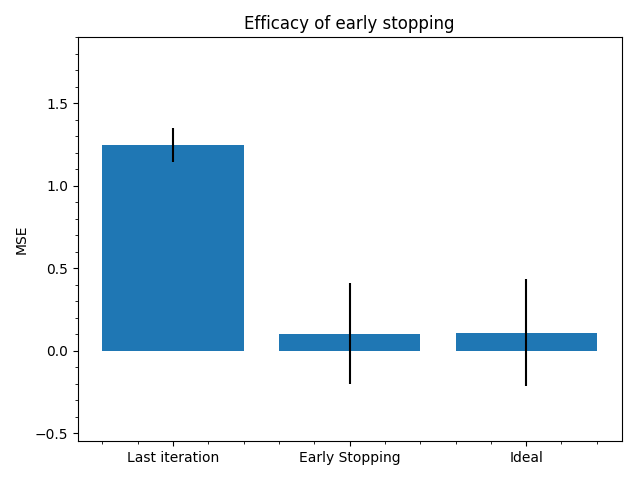
\includegraphics[scale=0.35]{plots/12b.png}
  \captionof{figure}{Early stopping.}
  \label{plot_simple_nh}
\end{figure}

\item \textbf{In the light of question 1.1.b) is it expected that early stopping happens (validation error is minimized) at the same iteration number for all random seeds? Is it coherent with your results?}
\newline \newline
It is not expected that early stopping happens at the same iteration number for all random seeds because of the different initial weights set by the random state parameter. This is also shown in our results.

\item \textbf{Early stopping in its standard form is a little different, instead of stopping when the validation error is minimized, one stops training as soon as the validation error increases. What are the pros and cons of those standard form of early stopping and the one you implemented?}
\newline \newline
The standard method of early stopping stops the training when the validation error increases, this is why this method can be faster but the validation error can be higher.
\end{itemize}

\newpage

\item \textbf{Combining the tricks:}\\
In the function ex\_1\_2\_c in file nn\_regression.py:
\begin{itemize}
\item Combining the results from all the previous questions, train a network with the ideal number of hidden neurons, regularization parameter and solver choice. Use 10 seeds, a validation set and early stopping to identify one particular network (a single seed) that performs optimally.
\end{itemize}
In your report:
\begin{itemize}
\item \textbf{Explain your choice of number of hidden neurons, regularization parameter and solver. Then describe in a short paragraph but rigorously the protocol followed to identify the optimal random seed (mention all the parameter you chose such as).}
\newline \newline
We decided to use 40 neurons for the calculation for reliable measurements because we used this amount of neurons for the previous calculations, so we are able to get valid and comparable data.
For the regularization parameter alpha we used \textit{$10^{-2}$} regarding the best value for alpha from exercise 1.2a.
By experimenting with different values for the solver and regularization parameter, we got to the conclusion that the solver \textit{lbfgs} delivered the best results for our purpose.
\newline \newline
During the iteration over the random seeds we calculate the MSE for the training, testing and validation sets 100 times.
We use early stopping to identify one particular network as mentioned in the assignment sheet. We then calculate the early stopping index in our MSE lists by using the \textit{argmin} function to evaluate the best matches.

\item \textbf{Report the mean and standard deviation of your training, validation and testing error. Report the training, validation and testing error of your optimal random seed.}
\newline \newline
\textbf{Mean Square Error Test:}
\begin{itemize}
\item Mean: \textit{1.1399337348359726}
\item Standard deviation: \textit{0.0023326551020294577}
\end{itemize}
\hfill \newline
\textbf{Mean Square Error Training:}
\begin{itemize}
\item Mean: \textit{1.0163030942948361}
\item Standard deviation: \textit{7.195428704528305e-05}
\end{itemize}
\hfill \newline
\textbf{Mean Square Error Validation:}
\begin{itemize}
\item Mean:\textit{ 0.9796973640162612}
\item Standard deviation: \textit{0.00038479446712075645}
\end{itemize}
\hfill \newline
\textbf{Optimal seed: 1}
\begin{itemize}
\item Training MSE with optimal seed:\textit{ 2}
\item Testing MSE with optimal seed: \textit{2}
\item Validation with optimal seed: \textit{1}
\end{itemize}

\end{itemize}
\end{enumerate}

\newpage

\section{Face Recognition with Neural Networks}

\subsection{Pose Recognition}
In the function ex\_2\_1 in file nn\_classification.py:
\begin{itemize}
	\item Write code to train a feed-forward neural network with 1 hidden layers containing 6 hidden units for pose recognition. Use dataset2 for training after normalization, ‘adam’ as the training solver and train for 200 iterations.
    \item Calculate the confusion matrix
    \item Plot the weights between each input neuron and the hidden neurons to visualize what the network has learnt in the first layer.
\end{itemize}
In your report:
\begin{itemize}

\item \textbf{Include the confusion matrix you obtain and discuss. Are there any poses which can be better separated than others?}
\newline \newline
The Confusion Matrix we obtained: 
\begin{table}[th]
\centering
\label{confusion_matrix_pose}
\begin{tabular}{|c|c|c|c|c|}
\hline
   & \textbf{Straight} & \textbf{Left} & \multicolumn{1}{l|}{\textbf{Right}} & \multicolumn{1}{l|}{\textbf{Up}} \\ \hline
\textbf{Straight} & 126                & 3             & 5                                   & 7                                \\ \hline
\textbf{Left}     & 1                 & 138           & 0                                   & 2                                \\ \hline
\textbf{Right}    & 1                 & 0             & 136                                 & 1                                \\ \hline
\textbf{Up}       & 11                & 4             & 1                                   & 128                              \\ \hline
\end{tabular}
\caption{Confusion Matrix}
\end{table}

\noindent
The higher the weight of the confusion matrix, the better the accuracy of the pose recognition. In our matrix we obtain high weights for \textit{left} and \textit{right} values. They have more accuracy than \textit{straight} or \textit{up}. But the accuracy for up and straight poses is still very accurate.

\item \textbf{Can you find particular regions of the images which get more weights than others?}
\newline \newline
In our confusion matrix, particular the \textit{left}, \textit{right}, \textit{straight} and the \textit{up} regions got more weights than others. The higher the diagonal values of the matrix, the more accuracy we have in our pose recognition.

\item \textbf{Include all plots in your report.} \\
\begin{minipage}{0.4\textwidth}
  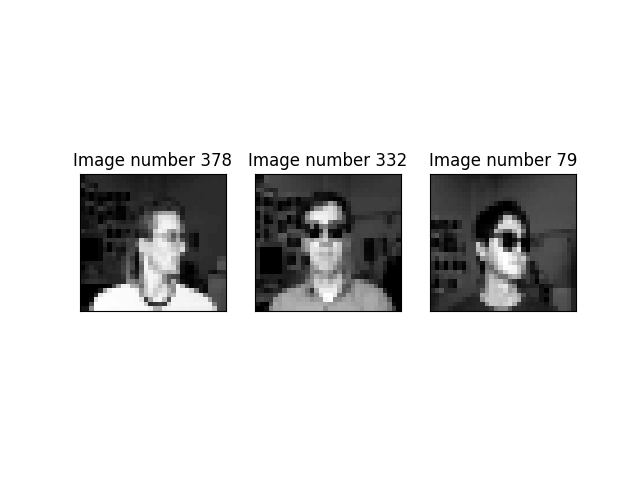
\includegraphics[scale=0.35]{plots/pose_recognition.png}
  \captionof{figure}{Recognized Poses}
  \label{pose_recognition}
\end{minipage}
\hfill
\begin{minipage}{0.4\textwidth}
  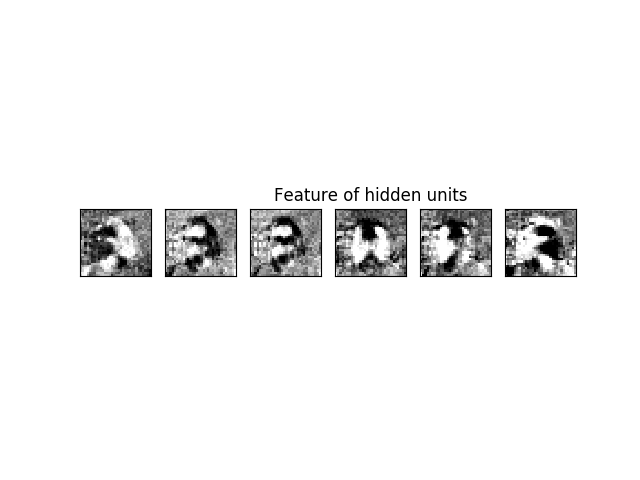
\includegraphics[scale=0.35]{plots/pose_recognition_hidden_units.png}
  \captionof{figure}{Weighted Regions}
  \label{pose_recognition_hidden_units}
\end{minipage}
\end{itemize}

\newpage

\subsection{Face Recognition}
In the function ex\_2\_2 in file nn\_classification.py:
\begin{itemize}
    \item Write code to train a feed-forward neural network with 1 hidden layer containing 20 hidden units for recognising the individuals. Use dataset1 for training, ‘adam’ as the training solver and train for 1000 iterations. Use dataset2 as the test set.
    \item Repeat the process 10 times starting from a different initial weight vector and plot the histogram for the resulting accuracy on the training and on the test set (the accuracy is proportion of correctly classified samples and it is computed with the method score of the classifier).
    \item Use the best network (with maximal accuracy on the test set) to calculate the confusion matrix for the test set.
	\item Plot a few misclassified images.
\end{itemize}
In your report:
\begin{itemize}
\item \textbf{Include all plots in your report.}

\begin{figure}[htp]
\centering
  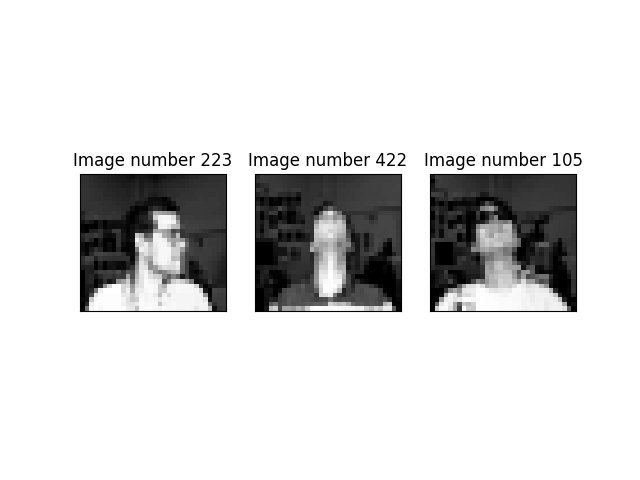
\includegraphics[scale=0.45]{plots/face_recognition.png}
  \caption{Face recognition with different poses.}
  \label{plot_simple_nh2}
\end{figure}

\begin{figure}[htp]
\centering
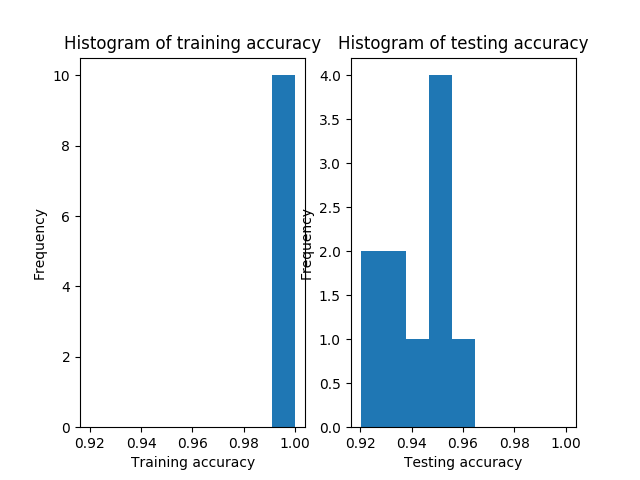
\includegraphics[scale=0.45]{plots/face_recognition_histogram.png}
  \caption{Accuracy histogram of training and testing set.}
  \label{plot_simple_nh8}
\end{figure}

\item \textbf{Why do different networks have different accuracies? Explain the variance in the results.}
\newline \newline
We computed networks with different initial weight vectors and so they differ in values and accuracy.
The accuracy of the training set is very close to 1.0 while we got some fluctuations in the testing set, where the accuracy is still very high with mostly 0.95.

\newpage

The Confusion Matrix we obtained: \\
\begin{table}[ht]
\centering
\label{my-label}
\begin{tabular}{llllllllllllllllllll}
27 & 0  & 0  & 0  & 0  & 0  & 2  & 0  & 0  & 0  & 0  & 0  & 0  & 0  & 0  & 0  & 0  & 0  & 0  & 0  \\
0  & 29 & 0  & 0  & 0  & 0  & 0  & 0  & 0  & 0  & 0  & 0  & 0  & 0  & 0  & 0  & 0  & 0  & 0  & 0  \\
0  & 0  & 28 & 0  & 0  & 0  & 0  & 0  & 0  & 0  & 0  & 0  & 0  & 0  & 0  & 0  & 0  & 0  & 0  & 0  \\
0  & 1  & 0  & 27 & 0  & 0  & 0  & 0  & 0  & 0  & 0  & 0  & 0  & 0  & 0  & 0  & 0  & 0  & 0  & 0  \\
0  & 0  & 0  & 0  & 24 & 3  & 0  & 0  & 0  & 0  & 0  & 0  & 0  & 0  & 0  & 0  & 0  & 0  & 0  & 0  \\
0  & 0  & 0  & 0  & 0  & 28 & 0  & 0  & 0  & 0  & 0  & 0  & 0  & 0  & 0  & 0  & 0  & 0  & 0  & 0  \\
0  & 0  & 0  & 0  & 0  & 8  & 19 & 0  & 0  & 1  & 0  & 0  & 0  & 0  & 0  & 0  & 0  & 0  & 0  & 0  \\
0  & 6  & 0  & 0  & 0  & 0  & 0  & 23 & 0  & 0  & 0  & 0  & 0  & 0  & 0  & 0  & 0  & 0  & 0  & 0  \\
0  & 0  & 0  & 0  & 0  & 0  & 0  & 0  & 29 & 0  & 0  & 0  & 0  & 0  & 0  & 0  & 0  & 0  & 0  & 0  \\
0  & 0  & 0  & 0  & 0  & 0  & 0  & 0  & 0  & 28 & 0  & 0  & 0  & 0  & 0  & 0  & 0  & 0  & 0  & 0  \\
0  & 0  & 0  & 0  & 0  & 0  & 0  & 0  & 0  & 0  & 28 & 0  & 0  & 0  & 0  & 0  & 0  & 0  & 0  & 0  \\
0  & 0  & 0  & 0  & 0  & 0  & 0  & 0  & 0  & 0  & 0  & 23 & 0  & 0  & 0  & 2  & 0  & 0  & 0  & 0  \\
0  & 0  & 0  & 0  & 0  & 0  & 0  & 0  & 0  & 0  & 0  & 0  & 29 & 0  & 0  & 0  & 0  & 0  & 0  & 0  \\
0  & 0  & 0  & 0  & 0  & 0  & 0  & 0  & 0  & 0  & 0  & 0  & 0  & 27 & 0  & 0  & 0  & 0  & 0  & 0  \\
0  & 0  & 0  & 0  & 0  & 0  & 0  & 0  & 0  & 0  & 0  & 0  & 0  & 0  & 29 & 0  & 0  & 0  & 0  & 0  \\
0  & 0  & 0  & 0  & 0  & 0  & 0  & 0  & 0  & 0  & 0  & 0  & 0  & 0  & 0  & 29 & 0  & 0  & 0  & 0  \\
0  & 0  & 0  & 0  & 0  & 0  & 0  & 0  & 0  & 0  & 0  & 0  & 0  & 0  & 0  & 0  & 27 & 0  & 0  & 0  \\
0  & 0  & 0  & 0  & 0  & 0  & 0  & 0  & 0  & 0  & 0  & 0  & 0  & 0  & 0  & 0  & 0  & 29 & 0  & 0  \\
0  & 0  & 0  & 0  & 0  & 0  & 0  & 0  & 0  & 0  & 0  & 0  & 0  & 0  & 0  & 0  & 0  & 0  & 29 & 0  \\
0  & 0  & 0  & 0  & 0  & 1  & 0  & 0  & 0  & 0  & 0  & 0  & 0  & 0  & 0  & 0  & 0  & 0  & 0  & 28
\end{tabular}
\caption{Confusion matrix generated by the network with the most accuracy on training set.}
\end{table}

\item \textbf{Do the misclassified images have anything in common?}

\begin{minipage}{0.4\textwidth}
  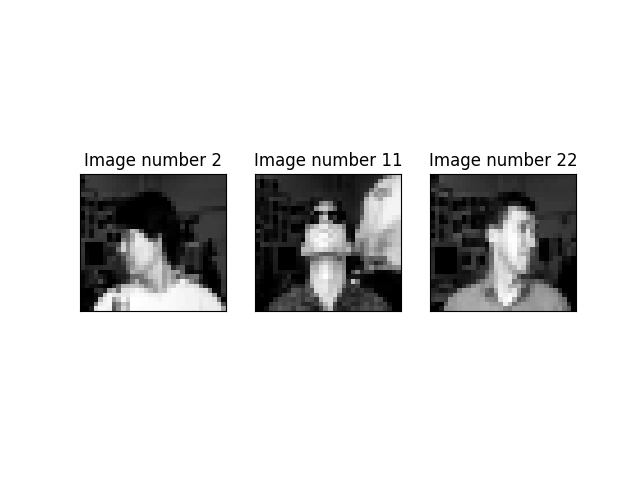
\includegraphics[scale=0.35]{plots/missclassified1.png}
  \captionof{figure}{Misclassified image set 1.}
  \label{plot_simple_nh2}
\end{minipage}
\hfill
\begin{minipage}{0.4\textwidth}
  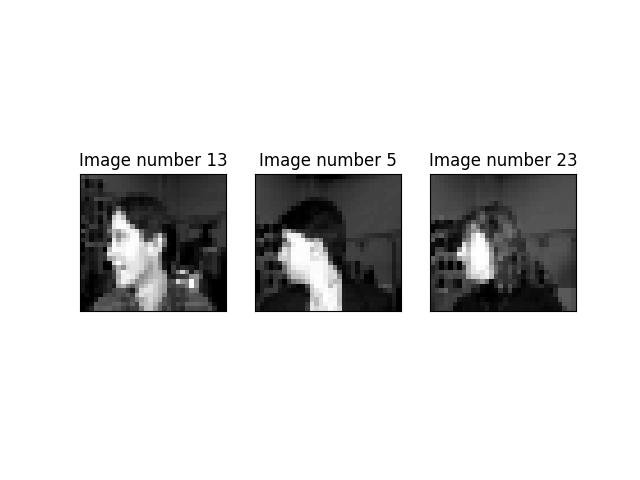
\includegraphics[scale=0.35]{plots/missclassified2.png}
  \captionof{figure}{Misclassified image set 2.}
  \label{plot_simple_nh8}
\end{minipage}

\begin{minipage}{0.4\textwidth}
  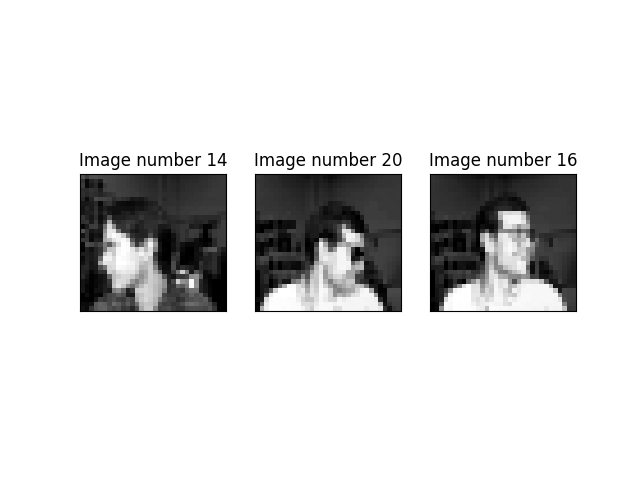
\includegraphics[scale=0.35]{plots/missclassified3.png}
  \captionof{figure}{Misclassified image set 3.}
  \label{plot_simple_nh2}
\end{minipage}
\hfill
\begin{minipage}{0.4\textwidth}
  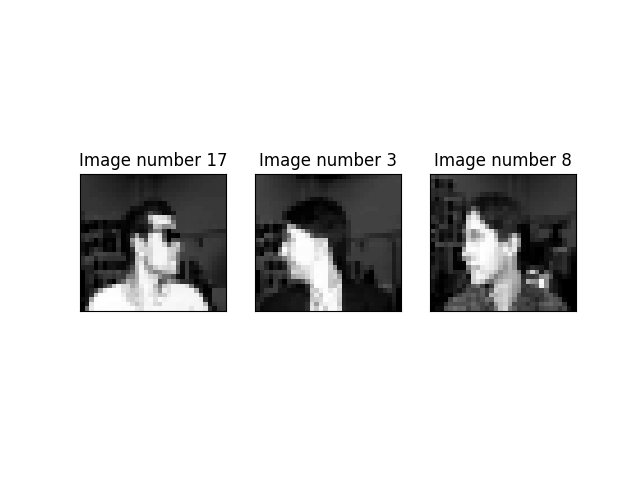
\includegraphics[scale=0.35]{plots/missclassified4.png}
  \captionof{figure}{Misclassified image set 4.}
  \label{plot_simple_nh8}
\end{minipage}
\newline \newline \newline
Some of the images are very equal to each other. Also the poses, especially \textit{left} and \textit{right} commonly appear in all misclassified image sets. 

\end{itemize}

%\section{Optional: Back-propagation with weight sharing}

\end{document}